\documentclass[11pt]{article}
\usepackage[a4paper, margin=20mm]{geometry}
\usepackage{wrapfig}
\usepackage{jtygm}
\usepackage{listings}
\usepackage[usenames, dvipsnames]{color}
\usepackage[dvipdfmx]{graphicx}
\usepackage{keystroke}
\usepackage{menukeys}
\usepackage{siunitx}

\newcommand\secref[1]{\mbox{Section~\ref{#1}}}
\newcommand\gamename{SamurAI Jockey}

\title{{\gamename} Game Rule}
\author{IPSJ Programming Contest Committee}
\date{2017/12/26}

\begin{document}
\maketitle

\begin{abstract}
  This document presents the game rules for SamurAI Coding 2017--18.
  % Note that this is a draft and is subject to change.
\end{abstract}

\section{Game Outline}
Two players controlled by AI programs, changing their positions step
by step, compete for time to goal in a course with obstacles.

One game consists of two races with the same course, exchanging the
start positions of two players.
The player with the smaller sum of goal times of two races wins the game.
If the goal time sums are equal, the game is a draw.

\begin{wrapfigure}{r}{0.38\columnwidth}
  \vspace{-2cm}
  \centering
  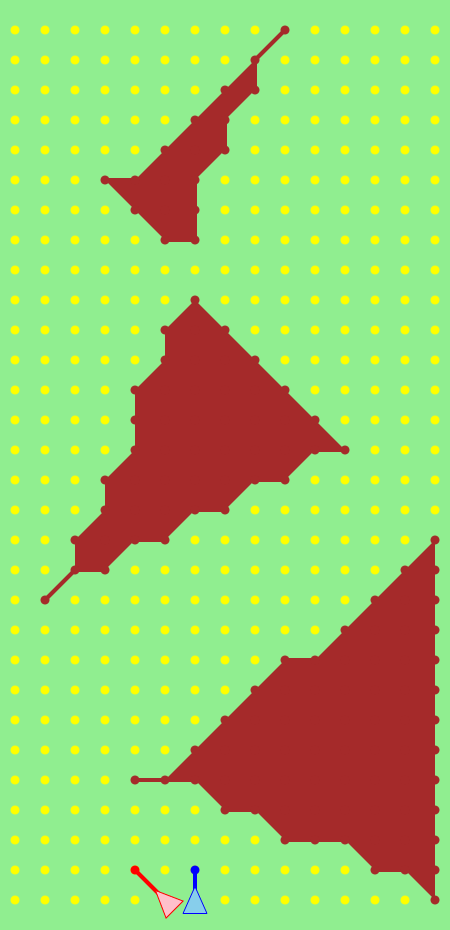
\includegraphics[width=0.35\columnwidth, natwidth=450, natheight=930]{racecourse.png}
  \caption{Race Course Example}
  \label{fig:course}
\end{wrapfigure}

\section{Race Course}
The race courses are a two dimensional grid, with different sizes and
obstacle positions for different games.  The width of the race course is
$w$ and its length is $l$ in what follows.  A grid point on the race
course has coordinates $(x,y)$ ($0\le x < w, 0\le y$).

Some of the grid points on the race course are {\em obstacle points.}
Obstacle points and line segments connecting them are {\em obstacles.}
Obstacles are fixed in one race.  The AI programs controlling players
(called {\em AI,} in what follows), however, are given information of
only those obstacles inside the players' fields of vision, that is,
those with their $y$-coordinates within a certain limit from the
$y$-coordinates of the players' positions.  As only limited
acceleration and deceleration are possible, obstacles may become
unavoidable with velocity too large.

Figure \ref{fig:course} shows an example of a race course.  The brown
dots are obstacle points, brown line segments are obstacles connecting
obstacle points, and the brown areas are those surrounded by obstacles
into which players cannot enter.

During one race, two players are on different grid points.  The start
points of two players are with $y$-coordinates of $0$ and different
$x$-coordinates.  As the race progresses, players change their
positions step by step.  Players finish the race when they have reached
a point with the $y$-coordinate greater than or equal to the course
length $l$.

There is never a dead end in the course.  A player can move to a point
with larger $y$-coordinate from any grid point of the race course that
can be reached from the start points of the two players, never
decreasing its $y$-coordinate during the move, if moves are with
velocity small enough.

\section{Race Process}\label{sec:race_process}
On every step of a race, both AI's are given information on the race
situation, and the situation is updated according to the
acceleration/deceleration instruction given by the players in
response.  Two players never occupy the same position at a time during
a race.

The race starts from step 0 and the step number is incremented one by
one.  The race ends when both of the players finish or become \emph{disqualified} (\secref{sec:disqualification}).  If one or more
players can't finish within the step limit, however, the race ends at
that step and the unfinished player is disqualified.

\subsection{Time Control}\label{sec:consideration_time}
A limit is imposed on the total of time a player can use in one race.
The clock starts or resumes when the game manager program has finished
sending information to the AI and stops when it has finished
receiving the response from the AI.  The player running out of
the time is disqualified.
% \footnote{The time limit is not fixed yet but is expected to be some
%   tens of seconds.}

\subsection{Player States and Acceleration Instructions}
A player has its {\em position} $(x, y)$ and {\em velocity} $(v_{\rm
  x}, v_{\rm y})$ at each step.

A player instructs {\em acceleration|} $(a_{\rm x}, a_{\rm y})$ at each step.
Both $a_{\rm x}$ and $a_{\rm y}$ should be one of $-1, 0,$ or $1.$

When the player can make normal move without committing course out and
collision with the opponent without priority (described below), the
position of the player at the next step will be $(x+v_{\rm x}+a_{\rm
  x}, y+v_{\rm y}+a_{\rm y})$.  This position is called the {\em
  planned position} in what follows.  The velocity of the player in
the next step will be $(v_{\rm x}+a_{\rm x}, v_{\rm y}+a_{\rm y})$
whether or not the player can make normal move.

\begin{wrapfigure}{R}{0.28\columnwidth}
  \vspace{-1cm}
  \centering
  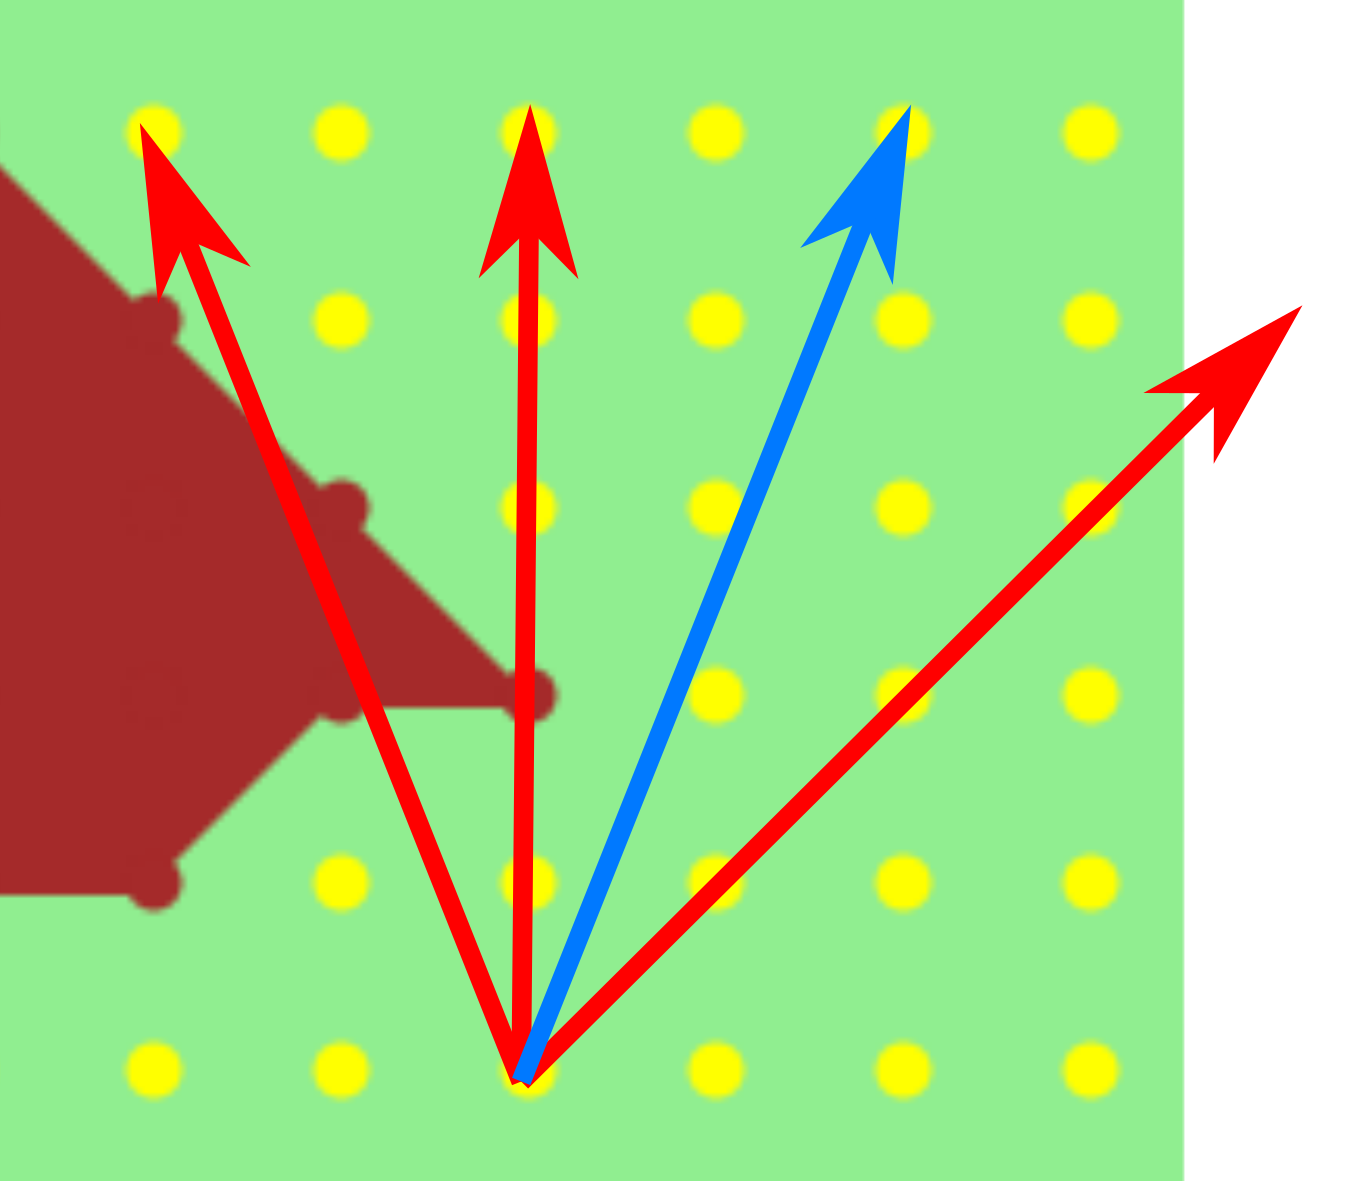
\includegraphics[width=0.26\columnwidth, natwidth=1358, natheight=1181]{courseout.png}
  \caption{Course Outs}
  \label{fig:courseout}
  Red movement lines cause course outs.
  \vspace{-1cm}
\end{wrapfigure}

\subsection{Movement Lines and Course Outs}
The line segment connecting the players position and its planned position is called the {\em movement line} of the player.

The player commits a {\em course out} if one or more of the
following hold.
\begin{itemize}
\item
  The player goes out of the course, that is, the coordinates of
  planned position $(x, y)$ does not satisfy both $0\le x<w$ and $0\le
  y.$
\item
  The movement line goes over or touches one or more obstacles.
\end{itemize}

The position of a player that committed a course out cannot move: its
position in the next step remains the same.  The acceleration is
applied the same as when no course outs are committed.

\begin{wrapfigure}{R}{0.32\columnwidth}
  \centering
  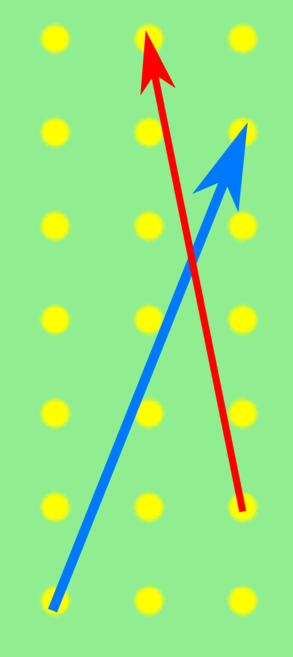
\includegraphics[scale=0.2, natwidth=293, natheight=657]{collision.png}
  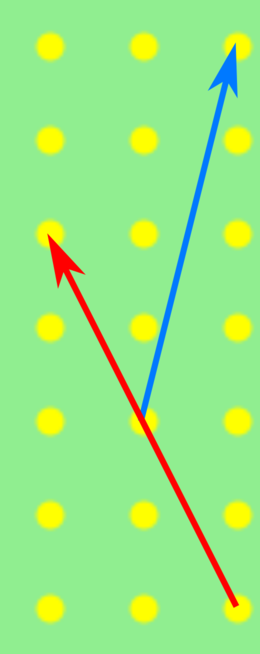
\includegraphics[scale=0.183, natwidth=288, natheight=657]{cropped.png}
  \caption{Collision}
  \label{fig:collision}
  The player with the blue movement line has the priority.
  \vspace{-1cm}
\end{wrapfigure}

\subsection{Collisions and Priorities}
When no course outs take place and movement lines of two players touch
or intersect, a {\em collision} takes place.

On a collision, the player with the {\em priority} will move to its
planned position, but one without the priority will be made to stay in
the same position.  The acceleration is applied the same as when no
collisions take place.

The player with the smaller $y$-coordinate of its position has the
priority.  When two players have the same $y$-coordinate, one with the
smaller $x$-coordinate has the priority.  An exception is when the
movement line of a player reaches or passes the opponent's original
position.  In this case, the priority is given to the opponent.

When movement lines of both players reaches or passes the opponents'
position, both lose the priority and cannot move at that step.

\subsection{Goal Time}
When a player at $(x, y)$ at step $s$ moves to $(x', y')$, and $y'\ge
l$ ($l$ is the course length) holds, that player finishes the race.
The goal time of the player is $s + (l-y)/(y'-y).$

A player that committed a course out or made a collision without
priority is stopped, and even if its planned position has
$y$-coordinate greater than or equal to the course length, the player
does not finish the race.
\footnote{Note that there may be obstacles on and beyond the goal line.}

The player that finished the race is removed from the course.  The
race continues if the opponent player has not finished the race or
been disqualified.

\subsection{Disqualification}\label{sec:disqualification}
A player is disqualified in either one of the following cases.
\begin{itemize}
\item The player can't finish within the step limit (the preface of \secref{sec:race_process}).
\item The player exceeds the time limit (\secref{sec:consideration_time}).
\item The output from the AI violates the regulations in Sections~\ref{sec:output_init} and \ref{sec:output_step}.
\end{itemize}

The disqualified player is removed from the course.  The race
continues if the opponent player has not finished the race or been
disqualified. The goal time of the disqualified player is twice the
step limit.

Note that the extent of the disqualification is limited to the current
race; the disqualified player can participate in subsequent races
without any penalties.

\section{Behavior of AI's}

The AI receives information related to the race as a whole at its
initiation, and responds with an acknowledgment of receiving it.  At
each step, it receives the race state information and responds with an
acceleration instruction.

The input of the AI is a sequence of decimal integers, separated by
one space or newline.  Negative values are prefixed with a minus
sign.  The initial game information and game state information at each
step end with a newline.

AI should respond sequences of decimal integers, separated by
spaces or a newline.  Negative values should be prefixed with a minus
sign.  {\bf A newline should be placed at the ends of responses.}

\subsection{Initial Input}
At initiation, an AI receives the following input items in this order.
A newline is put at the end of each item. Multiple integers within one item (line) are separated by {\bf one space character}.
\begin{description}
\item[Remaining Time ($t_\mathrm{given}$)] The remaining time usable in this race in
  microseconds as an integer.
\item[Step Limit ($s_\mathrm{max}$)] The limit of number of steps to finish as an integer.
\item[Course Size] The width ($w$) and length ($l$) of the race course as two integers.
\item[Vision Limit ($d$)] The depth of the field of vision as an integer
  $d$. When the player is at $(x, y)$, information of the opponent and
  obstacle points are given for those at $y$-coordinates between $y-d$
  and $y+d$, inclusive.
\end{description}

\makeatletter
\def\lst@visiblespace{$\color{Gray}{}_{
  \mbox{\kern.06em\vrule \@height.3ex}%
  \vbox{\hrule \@width.3em}%
  \hbox{\vrule \@height.3ex}}$}
\makeatother

\lstset{
  basicstyle=\ttfamily,
  frame = single,
  showspaces = true,
  escapeinside={<@}{@>},
  mathescape
}

\noindent
Following is the format of the initial input.

\begin{lstlisting}
$t_\mathrm{given}$<@\tiny{\keys{\return}}@>
$s_\mathrm{max}$<@\tiny{\keys{\return}}@>
$w$ $l$<@\tiny{\keys{\return}}@>
$d$<@\tiny{\keys{\return}}@>
\end{lstlisting}

\subsection{Initial Output}\label{sec:output_init}
An AI should respond with an integer $0$ and a newline to acknowledge that its
initiation is done.

\begin{lstlisting}
0<@\tiny{\keys{\return}}@>
\end{lstlisting}

\subsection{Per Step Input}
At each step, an AI receives the following items in this order.
A newline is put at the end of each item. Multiple integers included in one item are delimited by {\bf one space character}.
\begin{description}
\item[Step ($s$)] The current step number as a single integer.
\item[Remaining Time ($t_\mathrm{left}$)] The remaining time usable in this race in
  microseconds as an integer.
\item[Player's State] The $x$- and $y$-coordinates of the position ($x$ and $y$) and
  the $x$ and $y$ components the velocity $(v_\mathrm{x}$ and $v_\mathrm{y}$) of the player the AI is
  controlling, as four integers.
\item[Opponent's State] The $x$- and $y$-coordinates of the position ($x_\mathrm{e}$ and $y_\mathrm{e}$) and
  the $x$ and $y$ components the velocity ($v_{\mathrm{x}_\mathrm{e}}$ and $v_{\mathrm{y}_\mathrm{e}}$) of the opponent player, as
  four integers.  When the opponent player is out of the vision field,
  $-1$ is indicated for the $y$-coordinate of the position and $0$ for
  the remaining.
\item[Obstacle Points] Information on whether grid points in
  the vision field are obstacle points or not.  It consists of
  $(2\times d+1)\times w$ integers.  For every $y$ in the range
  $y_{\rm min} \le y \le y_{\rm max},$ $w$ integers $o_{0,y}, o_{1,y},
  \ldots, o_{w-1,y}$ are given.  $o_{x,y}$ being $1$ means that the
  grid point with its coordinates $(x,y)$ is an obstacle point, and
  $0$ means that it is not.  $1$ is given for grid points out of the
  course, that are, those with $y<0$.  A newline is used as a
  delimiter instead of a space character between $o_{w-1,y}$ and $o_{0,y+1}$.
  Thus, this information consists of integers of $2 \times d + 1$ rows by $w$ columns.

\end{description}

\noindent
The following is the format of the per step input.

\begin{lstlisting}
$s$<@\tiny{\keys{\return}}@>
$t_\mathrm{left}$<@\tiny{\keys{\return}}@>
$x$ $y$ $v_\mathrm{x}$ $v_\mathrm{y}$<@\tiny{\keys{\return}}@>
$x_\mathrm{e}$ $y_\mathrm{e}$ $v_{\mathrm{x}_\mathrm{e}}$ $v_{\mathrm{y}_\mathrm{e}}$<@\tiny{\keys{\return}}@>
$o_{0,y-d}$ $o_{1,y-d}$ $\ldots$ $o_{w-1,y-d}$<@\tiny{\keys{\return}}@>
$o_{0,y-d+1}$ $o_{1,y-d+1}$ $\ldots$ $o_{w-1,y-d+1}$<@\tiny{\keys{\return}}@>
$\ldots$
$o_{0,y+d}$ $o_{1,y+d}$ $\ldots$ $o_{w-1,y+d}$<@\tiny{\keys{\return}}@>
\end{lstlisting}

\subsection{Per Step Output}\label{sec:output_step}
An AI should output $x$- and $y$-components of the
acceleration at the clock with two integers $a_{\rm x}$ and $a_{\rm
  y}$ as two integers.
$a_{\rm x}$ and $a_{\rm y}$ should be one of $-1$, $0$, or $1$.
The integers should be delimited by one or more space characters, and a newline should be put after them.
The following is the format of the per step output.
Note that there can be more than one space characters between $a_\mathrm{x}$ and $a_\mathrm{y}$.

\begin{lstlisting}
$a_{\rm x}$ $a_{\rm y}$<@\tiny{\keys{\return}}@>
\end{lstlisting}

\subsection{Input and Output Example}

\newlength\defaultparindent
\defaultparindent=\parindent

\begin{minipage}[t]{.6\textwidth}

The text on the right is an example of the input/output to/from an AI
during the initiation and the first two steps.
The black text is the input and the red one is the output.

\parindent=\defaultparindent

The first four lines, being the initial input, indicate that
the remaining time, step limit, course width, course length and vision limit
are $20,000\,\si{\micro\second}$, 100, 15, 100 and 8 respectively.

When the AI receives this input, it should output 0 and a newline.

Then the AI receives the input of the first step.
0 and 19981 in the first two lines show the current step number
and the remaining time, respectively.
The AI can see that it took $19\,\si{\micro\second}$ for its initiation and
$19,981\,\si{\micro\second}$ remain.

The next two lines show the state of this and the opponent AI players.
The current position $(x,y)$ and the velocity $(v_\mathrm{x},v_\mathrm{y})$ of this player are $(5,0)$ and
$(0,0)$, respectively.
The position $(x_\mathrm{e},y_\mathrm{e})$ and the velocity $(v_{\mathrm{x}_\mathrm{e}},v_{\mathrm{y}_\mathrm{e}})$ of the opponent player are
$(9,0)$, and $(0,0)$, respectively.

The next 17 ($=8 \times 2 + 1$ because the vision limit is 8) lines give the information on whether grid points in the vision field are obstacle points or not.
It is discovered that all the grid points where $y < 0$ are obstacle points
and there is a large obstacle object straight in front of the player.

When the AI receives the input, it should output two integers as an acceleration $(a_\mathrm{x}, a_\mathrm{y})$;
it output $(-1,1)$ in this example.
Then the AI receives the input of the second step
in the same format to the first step.
Then the AI should output an acceleration again.
Such inputs and outputs are repeated until the race ends.

\end{minipage}
 \hfill
\begin{minipage}[t]{.3\textwidth}
\begin{lstlisting}[aboveskip = -1.4\medskipamount, showspaces = false, basicstyle = \tiny, literate = {-}{-}1]
20000
100
15 100
8
<@\textcolor{red}{0}@>
0
19981
5 0 0 0
9 0 0 0
1 1 1 1 1 1 1 1 1 1 1 1 1 1 1
1 1 1 1 1 1 1 1 1 1 1 1 1 1 1
1 1 1 1 1 1 1 1 1 1 1 1 1 1 1
1 1 1 1 1 1 1 1 1 1 1 1 1 1 1
1 1 1 1 1 1 1 1 1 1 1 1 1 1 1
1 1 1 1 1 1 1 1 1 1 1 1 1 1 1
1 1 1 1 1 1 1 1 1 1 1 1 1 1 1
1 1 1 1 1 1 1 1 1 1 1 1 1 1 1
0 0 0 0 0 0 0 0 0 0 0 0 0 0 0
0 0 0 0 0 0 0 0 0 0 0 0 0 0 0
0 0 0 0 0 0 0 1 0 0 0 0 0 0 0
0 0 0 0 0 0 0 1 0 0 0 0 0 0 0
0 0 0 0 0 0 1 1 0 0 0 0 0 0 0
0 0 0 0 0 0 1 1 1 0 0 0 0 0 0
0 0 0 0 0 1 1 1 1 0 0 0 0 0 0
0 0 0 0 0 1 1 1 1 0 0 0 0 0 0
0 0 0 0 1 1 1 1 1 1 0 0 0 0 0
<@\textcolor{red}{-1 1}@>
1
19955
4 1 -1 1
8 1 -1 1
1 1 1 1 1 1 1 1 1 1 1 1 1 1 1
1 1 1 1 1 1 1 1 1 1 1 1 1 1 1
1 1 1 1 1 1 1 1 1 1 1 1 1 1 1
1 1 1 1 1 1 1 1 1 1 1 1 1 1 1
1 1 1 1 1 1 1 1 1 1 1 1 1 1 1
1 1 1 1 1 1 1 1 1 1 1 1 1 1 1
1 1 1 1 1 1 1 1 1 1 1 1 1 1 1
0 0 0 0 0 0 0 0 0 0 0 0 0 0 0
0 0 0 0 0 0 0 0 0 0 0 0 0 0 0
0 0 0 0 0 0 0 1 0 0 0 0 0 0 0
0 0 0 0 0 0 0 1 0 0 0 0 0 0 0
0 0 0 0 0 0 1 1 0 0 0 0 0 0 0
0 0 0 0 0 0 1 1 1 0 0 0 0 0 0
0 0 0 0 0 1 1 1 1 0 0 0 0 0 0
0 0 0 0 0 1 1 1 1 0 0 0 0 0 0
0 0 0 0 1 1 1 1 1 1 0 0 0 0 0
0 0 0 1 1 1 1 1 1 1 0 0 0 0 0
<@\textcolor{red}{0 1}@>
\end{lstlisting}
\end{minipage}

\subsection{Memory Duration}
At each step, the game management system suspends the execution of AI
when receiving its output has been completed, and resumes it after
giving per step information.  Thus AI cannot continue its computation
between steps but its execution context, including variable values,
are kept during one whole race.

For each race, the game management system initiates AI from scratch in
an environment in which file I/O and network accesses are disabled.
Thus, AI cannot pass information between multiple races.

\end{document}
